\documentclass[11pt, a4paper]{article}
\usepackage{polski}
\usepackage[utf8]{inputenc}

\usepackage{amssymb}
\usepackage{amsmath}
\usepackage[pdftex]{graphicx}
\usepackage[margin=2.5cm]{geometry}

\usepackage{algorithm2e}
\usepackage{algorithmic}
\usepackage{mathtools}
\usepackage{hyperref}
\usepackage{tikz}
\usepackage{tkz-euclide}
\usetkzobj{all} 

\title{Dokumentacja projektu nr 1 z Grafiki Komputerowej I  \\
      ,,Edytor wielokątów''}
\author{Jadwiga Słowik gr. C1}

\begin{document}
 \maketitle
 \section{Instrukcja obsługi}
 Program zapewnia użytkownikowi cztery tryby pracy:
 \begin{enumerate}
  \item \hyperlink{AddNewPolygon}{Dodawanie nowego wielokąta}
  \item \hyperlink{AddNewVertex}{Dodawanie nowego wierzchołka do wielokąta}
  \item \hyperlink{Select}{Tryb zaznaczania} (oraz \hyperlink{Move}{przesuwanie} i \hyperlink{Delete}{usuwanie})
  \item \hyperlink{Relation}{Tryb ustawienia ograniczenia (tzw. ,,relacji'')}
    
 \end{enumerate}
 
 \hypertarget{AddNewPolygon}{\subsection{Dodawanie nowego wielokąta}}
 Użytkownik dodaje nowy wielokąt wyznaczając położenie jego kolejnych wierzchołków. Każde pojedyncze kliknięcie
 lewym przyciskiem myszy wyznacza kolejny punkt. Aby~dodawanie wielokąta zostało ukończone, pierwszy wierzchołek musi być
 taki sam jak~ostatni.
 
 Program uniemożliwia użytkownikowi stworzenie wielokąta, w~którym wierzchołki powtarzają~się (oprócz
 początkowego i~końcowego wierzchołka).
 
 Zakładamy, że~wielokąt musi mieć co~najmniej trzy wierzchołki. Nie~można utworzyć ,,wielokąta'' składającego~się
 z~jednego lub~dwóch~wierzchołków.
 
 Użytkownik ma~również możliwość cofania pojedynczych operacji dodawania wierzchołków poprzez~pojedyncze kliknięcie
 prawym przyciskiem myszy (w~dowolnym miejscu panelu do~rysowania).
 Nie jest możliwe cofnięcie ostatniej operacji, jeśli~tworzenie wielokąta zostało ukończone
 (użytkownik kliknął na~węzeł początkowy).
 
 Niemożliwe jest również wyjście z~tego trybu w~trakcie dodawania nowego wielokąta. Jeśli~użytkownik chce anulować dodawanie
 (nieukończonego) nowego wielokąta, może~to zrobić na~dwa sposoby:
 \begin{enumerate}
  \item Pojedynczo cofać każdą operację poprzez~klikanie prawym przyciskiem myszy
  \item Ukończyć dodawanie wielokąta klikając na~pierwszy wierzchołek, a~następnie przejść do~trybu \hyperlink{Select}{Zaznaczania}
      i~usunąć cały wielokąt
 \end{enumerate}
 
 \hypertarget{AddNewVertex}{\subsection{Dodawanie nowego wierzchołka do wielokąta}}
 Użytkownik może dodać nowy wierzchołek do~istniejącego wielokąta klikając lewym przyciskiem myszy
 w~dowolne miejsce wybranej krawędzi.
 Wówczas, wierzchołek pojawi~się na~środku wybranej krawędzi bez~względu na~rzeczywiste miejce kliknięcia myszą.
 
 Krawedź, na~której nowy wierzchołek został dodany, traci ustanowione wcześniej ograniczenie (,,relację'').
 
 \hypertarget{Select}{\subsection{Tryb zaznaczania}}
 W~tym trybie użytkownik może zaznaczyć wybrany wielokąt klikając na~nim prawym przyciskiem myszy.
 Istnieją trzy różne sposoby zaznaczenia wielokąta:
 \begin{enumerate}
    \item Pojedyncze kliknięcie prawym przyciskiem myszy na~wierzchołek zaznacza tylko wierzchołek
    \item Pojedyncze kliknięcie prawym przyciskiem myszy na~krawędź zaznacza tylko krawędź
    \item Podwójne kliknięcie prawym przyciskiem myszy na~wierzchołku lub krawędzi zaznacza całą figurę
 \end{enumerate}
 Po zaznaczeniu figury (lub jej części) zmienia ona (lub jej część) kolor na zielony.
 Wówczas, możliwa jest modyfikacja zaznaczonego wielokąta:
 \begin{enumerate}
  \item \hypertarget{Move}{Przesuwanie wybranego wierzchołka/figury} \\
    Przesuwanie obiektu jest możliwe jedynie wtedy, gdy~jest zaznaczony.
    Klikamy lewym przyciskiem myszy na~zaznaczoną część
    i~trzymając cały czas wciśnięty przycisk myszy przesuwamy obiekt w~wybrane miejsce. 
    Wraz~z~przesuwaniem kursora myszy cały czas widoczna jest zmiana położenia figury (lub tylko części).
  \item \hypertarget{Delete}{Usuwanie wybranego wierzchołka/krawędzi/figury} \\
    Usuwanie obiektu jest możliwe jedynie wtedy, gdy~jest zaznaczony.
    Aby~usunąć wybraną wcześniej figurę (lub~jej część)
    należy dwukrotnie kliknąć lewym przyciskiem myszy w~dowolne miejsce panelu do~rysowania.
    
    Jeśli usuwamy wierzchołek lub~krawędź trójkąta, to, w~rezultacie, zostanie~usunięty cały wielokąt,
    gdyż~na~mocy postawionych wcześniej założeń, figura~jedno- lub dwu- wierzchołkowa nie~jest traktowana
    jako~wielokąt.
 \end{enumerate}
 Istnieje możliwość zaznaczenia wybranej figury (lub jej fragmentu) i~przejście do~innego trybu. Zaznaczenie wówczas
 nie~zniknie. 
 
 Jeśli użytkownik będzie chciał odznaczyć zaznaczony wcześniej obiekt, 
 może~tego dokonać klikając prawym przyciskiem myszy
 w~dowolne puste miejsce panelu do~rysowania (ważne jest, aby~był w~trybie zaznaczania; w~innym trybie owa operacja
 nie~przyniesie pożądanego skutku).
 
 \hypertarget{Relation}{\subsection{Tryb ustawienia ograniczenia (,,relacji'')}}
 W~tym miejscu możemy ustawić ograniczenia dla~wybranych krawędzi.
 
 Aby~ustawić ograniczenie dla~wybranej krawędzi, należy kliknąć na~nią lewym przyciskiem myszy.
 Wówczas, powinno pojawić się nowe okienko, gdzie~użytkownik może wybrać ograniczenie, które~go interesuje.
 Istnieją trzy rodzaje ograniczeń:
 \begin{enumerate}
  \item Stała zmiana krawędzi na~pionową
  \item Stała zmiana krawędzi na~poziomą
  \item Stała zmiana długości krawędzi na~podaną przez~użytkownika wartość
 \end{enumerate}
 Po~zatwierdzeniu operacji, na~wybranej krawędzi powinna pojawić~się odpowiednia ikonka symbolizująca ustawioną ,,relację''.
 Ustawienie ograniczenia może powodować nie~tylko zmianę położenia wybranej krawędzi, ale~również zmianę ustawienia
 pewnej grupy innych krawędzi, jeśli~będzie to~konieczne, aby~wszystkie ustawione ograniczenia dla~danego wielokąta
 pozostały spełnione.
 
 Jeśli wybrana relacja nie~jest możliwa do~ustawienia, użytkownik zostanie o~tym poinformowany poprzez~odpowiedni komunikat
 programu i~operacja zostanie anulowana.  Każda krawędź może mieć ustawione maksymalnie jedno ograniczenie oraz~nie~może być dwóch sąsiadujących ze~sobą krawędzi
 poziomych lub pionowych.
 
 Aby usunąć ustanowione wcześniej ograniczenie, należy kliknąć prawym przyciskiem myszy na~wybraną krawędź.
 
 
 \section{Opis algorytmu ,,relacji''}
 Po~ustawieniu ograniczenia dla~danej krawędzi może wystąpić konieczność zmiany jej położenia.
 \begin{enumerate}
  \item Jeśli ma~być pionowa, to rozważamy następujące dwie opcje --- zmianę położenia pierwszego lub~drugiego końca krawędzi \\ \\
  \begin{tikzpicture}
   \draw (0,0) -- (3,3);
   \node(A) at (0,0) {\pgfuseplotmark{*}};
   \node(B) at (3,3) {\pgfuseplotmark{*}};
   
   \draw[red, dashed] (0,0) -- (0,3);
   \node(P1)[red] at (3,0) {\pgfuseplotmark{*}};
   \node(NP1)[above right = 2pt, outer sep=2pt,fill=white] at (3,0) {$P_1$};
   
   \draw[blue, dashed] (3,3) -- (3,0);
   \node(P2)[blue] at (0,3) {\pgfuseplotmark{*}};
   \node(NP2)[left = 2pt, outer sep=2pt,fill=white] at (0,3) {$P_2$};
   
   \draw[->, to path={-- (\tikztotarget)}]
    (A) edge (P1);
   \draw[->, to path={-- (\tikztotarget)}]
    (B) edge (P2);
   
  \end{tikzpicture} \\
  Tym samym, przekształcamy początkową, czarną krawędź do~niebieskiej lub czerwonej krawędzi.
  \item Jeśli krawędź ma~być pozioma, to postępujemy analogicznie do~przypadku z~krawędzią pionową \\ \\
  \begin{tikzpicture}
   \draw (0,0) -- (3,3);
   \node(A) at (0,0) {\pgfuseplotmark{*}};
   \node(B) at (3,3) {\pgfuseplotmark{*}};
   
   \draw[red, dashed] (0,0) -- (3,0);
   \node(P1)[red] at (3,0) {\pgfuseplotmark{*}};
   \node(NP1)[above right = 2pt, outer sep=2pt,fill=white] at (3,0) {$P_1$};
   
   \draw[blue, dashed] (3,3) -- (0,3);
   \node(P2)[blue] at (0,3) {\pgfuseplotmark{*}};
   \node(NP2)[left = 2pt, outer sep=2pt,fill=white] at (0,3) {$P_2$};
   
   \draw[->, to path={-| (\tikztotarget)}]
    (A) edge (P2);
   \draw[->, to path={-| (\tikztotarget)}]
    (B) edge (P1);
  \end{tikzpicture}
 \item Jeśli ma mieć ustaloną długość, to~najpierw rozszerzamy/skracamy ją w~taki sposób, że~kierunek prostej,
       na~której leży dana krawędź, pozostaje taki sam. Gdyby okazało~się,
       że przy~zachowaniu kierunku krawędzi, ustawienie relacji jest niemożliwe, to~sprawdzamy kolejno każdy z~punktów
       leżących na~okręgach o~środkach w~końcach krawędzi i~promieniu równym podanej przez~użytkownika długości krawędzi.

 \end{enumerate} 
Zauważmy, że~ustawienie ograniczenia dla~krawędzi może spowodować konieczność zmiany położenia pewnej grupy innych punktów
 należących do~wielokąta. ,,Naprawę'' pozostałych ograniczeń będziemy wykonywać w~następujący sposób: \\ \\
 W~zależności od~tego, który~koniec krawędzi ulegnie zmianie, będziemy odwiedzać wierzchołki w~kolejności zgodnej
 z~ruchem wskazówek zegara
 lub~przeciwnej do~ruchu wskazówek zegara.
 \newpage \noindent
 W~celu ustalenia uwagi spójrzmy na~poniższy przykład. Przypuśćmy, że~zmieniamy położenie
 wierzchołka $0$ w~celu ustawienia ,,relacji'' poziomej na~krawędzi $0 - 3$.
 
 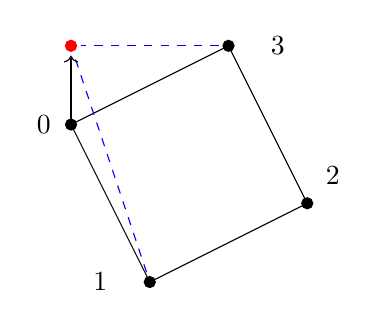
\begin{tikzpicture}
  \draw (0,0) -- (2,1);
  \node(A) at (0,0) {\pgfuseplotmark{*}};
   \node(NA)[left = 2pt, outer sep=2pt,fill=white] at (0,0) {$0$};
   
  \node(B) at (2,1) {\pgfuseplotmark{*}};
   \node(NB)[ right = 10pt, outer sep=2pt,fill=white] at (2,1) {$3$};
  
  \draw (2,1) -- (3,-1);
   \node(C) at (3,-1) {\pgfuseplotmark{*}};
   \node(NC)[above right = 2pt, outer sep=2pt,fill=white] at (3,-1) {$2$};
   
  \draw (3,-1) -- (1,-2);
   \node(D) at (1,-2) {\pgfuseplotmark{*}};
   \node(ND)[left = 10pt, outer sep=2pt,fill=white] at (1,-2) {$1$};
   
  \draw (1,-2) -- (0,0);
  
  \node[red](X) at (0,1) {\pgfuseplotmark{*}};
  %\node(VP)[left = 5pt, outer sep=2pt,fill=white] at (2,0) {$v'$};
  \draw[blue, dashed] (B) -- (X);
  \draw[blue, dashed] (D) -- (X);
  
   \draw[->, to path={-| (\tikztotarget)}]
    (A) edge (X);
 \end{tikzpicture} \\
 Poruszamy się w~kierunku krawędzi, która~ulega zmianie po~przesunięciu wierzchołka i~może już nie~spełniać danego jej wcześniej
 ograniczenia.  Zauważmy, że~krawędź $0 - 3$ jest~poprawnie ustawiona. Natomiast druga krawędź -- $0 - 1$ -- niekoniecznie.
 W~ogólności, dążymy do~tego, aby~,,naprawić'' aktualnie rozważaną krawędź w~taki sposób, aby~owa zmiana nie~zmieniła
 położenia kolejnej krawędzi. Jeśli osiągnięcie tego celu jest niemożliwe, przesuwamy~aktualnie rozważany wierzchołek
 o~taki sam wektor, o~jaki został przesunięty poprzedni wierzchołek i~przechodzimy do~kolejnej
 krawędzi, próbując zmienić położenie kolejnego wierzchołka (o~ile owe~przesunięcie spowodowało, że~,,relacja'' na~kolejnej
 krawędzi nie~jest już spełniona), itd.
 
 Próbujemy zmieniać położenie kolejnych wierzchołków wielokąta dopóki, dopóty~zmiana położenia danego wierzchołka
 zaburza ustawioną ,,relację'' dla~kolejnej krawędzi lub~dojdziemy do~wierzchołka, który~jest końcem krawędzi,
 którą~zmienialiśmy na~samym początku (w~celu ustanowienia nowego ograniczenia) -- jeśli wystąpi konieczność zmiany
 położenia drugiego końca krawędzi, na~której ustawiamy ograniczenie, to~znaczy, że~operacja ustawienia ograniczenia jest~niemożliwa do~wykonania.
 
 W~zależności od~ustawionej relacji na~aktualnie ,,naprawianej'' krawędzi, podejmujemy odpowiednie kroki.
 Przypuśćmy, że~aktualnie naprawiana~krawędź (o~indeksie $s$) ma~ustawione ograniczenie ($v$ -- indeks aktualnie rozważanego, w~celu zmiany
 położenia, wierzchołka. Załóżmy, że~poruszamy~się przeciwnie do~ruchu wskazówek zegara. Procedura, w~której poruszamy~się
 zgodnie z~ruchem wskazówek zegara, jest~analogiczna, zmieniają~się jedynie numery indeksów):
 \begin{enumerate}
  \item Krawędzi poziomej  \\
    Jeśli wektor przesunięcia dla~poprzedniego wierzchołka jest wektorem poziomym, to~możemy od~razu zakończyć
    procedurę (przesunięcie jednego z~końców krawędzi poziomej o~wektor nie~spowoduje w~żadnym wypadku zmiany
    orientacji owej krawędzi).
    Jeśli nie~jest poziomy, sprawdzamy, jakie ograniczenie jest ustawione na~$(s + 1)$-tej krawędzi. Mogą zajść następujące przypadki:
    \begin{enumerate}
     \item Krawędź $(s + 1)$-sza nie~ma ustawionej ,,relacji'' \\
     Przesuwamy $v$-ty wierzchołek o~ten sam wektor, o~który został przesunięty poprzedni wierzchołek i~kończymy całą procedurę.
     \item Krawędź $(s + 1)$-sza ma ustawioną ,,relację'' pionową \\
     \begin{tikzpicture}
       \node(A) at (0,0) {\pgfuseplotmark{*}};
       \node(NA)[above left = 2pt, outer sep=2pt,fill=white] at (0,0) {$v-1$};
       
       \node(B) at (2,1) {\pgfuseplotmark{*}};
       \node(NB)[above left = 2pt, outer sep=2pt,fill=white] at (2,1) {$v$};
       
       \draw (A) -- (B);
       
       \node(C) at (2, -2) {\pgfuseplotmark{*}};
       \node(NC)[above left = 2pt, outer sep=2pt,fill=white] at (2,-2) {$v+1$};
       
       \draw (B) -- (C);
       
       \node(P1)[red] at (2, 0) {\pgfuseplotmark{*}};
       \node(VP)[left = 5pt, outer sep=2pt,fill=white] at (2,0) {$v'$};
       \draw[blue,dashed] (A) -- (P1);
       \draw[blue,dashed] (C) -- (P1);
       
     \end{tikzpicture} \\
     Wówczas musimy przesunąć aktualnie rozważany wierzchołek o~wektor pionowy w~taki sposób, aby~współrzędna $y$ obecnie
     przetwarzanego wierzchołka była taka sama jak współrzędna $y$ poprzedniego (przesuniętego) wierzchołka
     (aby~naprawić ,,relację'' poziomą
     dla~$s$-tej krawędzi i~równocześnie nie~zaburzyć relacji pionowej dla~$(s+1)-szej$ krawędzi). Po~wykonaniu tej operacji,
     możemy zakończyć całą procedurę.
     \item \hypertarget{HorLen}{Krawędź $(s+1)$-sza ma~ustawioną ,,relację'' długości ($L$ -- ustalona długość)} \\
     \begin{tikzpicture}
       \node(A) at (0,0) {\pgfuseplotmark{*}};
       \node(NA)[above left = 2pt, outer sep=2pt,fill=white] at (0,0) {$v-1$};
       
       \node(B) at (2,1) {\pgfuseplotmark{*}};
       \node(NB)[above left = 2pt, outer sep=2pt,fill=white] at (2,1) {$v$};
       
       \draw (A) -- (B);
       
       \node(C) at (3, -2) {\pgfuseplotmark{*}};
       \node(NC)[above left = 2pt, outer sep=2pt,fill=white] at (3,-2) {$v+1$};
       
       \draw (B) -- (C);
	
       \draw[green, dashed] (-1,0) -- (6, 0);
       
       \draw (C) circle [radius=3.15];
       
       \node(P1)[red] at (0.55, 0) {\pgfuseplotmark{*}};
       \node(VP)[right = 5pt, outer sep=2pt,fill=white] at (0.55,0) {$v'$};
       \node(P2)[red] at (5.45, 0) {\pgfuseplotmark{*}};
       
       \draw[blue, dashed](A) -- (P1);
       \draw[blue, dashed](C) -- (P1);
      \end{tikzpicture} \\
      Znajdujemy punkty przecięcia prostej $x = vertex[s-1].X$ z~okręgiem $(vertex[s+1],\, L)$. Wierzchołek $v$-ty możemy
      przesunąć do~dowolnego z~punktów przecięcia (o~ile istnieje co~najmniej jeden) i~zakończyć procedurę.
      Jeśli nie~ma ani~jednego punktu przecięcia, to~przesuwamy $v$-ty wierzchołek o~ten sam wektor, o~jaki został przesunięty
      poprzedni wierzchołek i~przechodzimy do~następnego wierzchołka. \\
      
    \end{enumerate}
    \item Krawędzi pionowej \\
    Jeśli wektor przesunięcia poprzedniego wierzchołka jest wektorem pionowym, to~możemy w~tym momencie zakończyć procedurę.
    Jeśli nie~jest pionowy, musimy rozważyć następujące przypadki odnośnie następujące przypadki zależne od~postaci krawędzi
    $(s+1)-szej$
    \begin{enumerate}
     \item Krawędź $(s+1)$-sza nie~ma ustawionej relacji \\
     Wówczas przesuwamy wierzchołek $v$-ty o~ten sam wektor, o~jaki został przesunięty poprzedni wierzchołek i~kończymy procedurę.
     \item Krawędź $(s+1)$-sza ma~ustawioną relację poziomą \\
       \begin{tikzpicture}
       \node(A) at (0,0) {\pgfuseplotmark{*}};
       \node(NA)[above left = 2pt, outer sep=2pt,fill=white] at (0,0) {$v-1$};
       
       \node(B) at (1,2) {\pgfuseplotmark{*}};
       \node(NB)[above left = 2pt, outer sep=2pt,fill=white] at (1,2) {$v$};
       
       \draw (A) -- (B);
       
       \node(C) at (3,2) {\pgfuseplotmark{*}};
       \node(NC)[above left = 2pt, outer sep=2pt,fill=white] at (3,2) {$v + 1$};
       
       \draw (B) -- (C);
       
       \node[red](P1) at (0, 2) {\pgfuseplotmark{*}};
       \node(VP)[left = 5pt, outer sep=2pt,fill=white] at (0,2) {$v'$};
       \draw[blue, dashed] (A) -- (P1);
       \draw[blue, dashed] (C) -- (P1);
       \end{tikzpicture} \\
       Wówczas, musimy przesunąć $v$-ty wierzchołek o~wektor poziomy tak, aby~$s$-ta krawędź stała~się krawędzią poziomą.
       Następnie, możemy zakończyć całą procedurę.
     \item \hypertarget{VerLen}{$(s+1)-sza$ ma~ustaloną relację długości ($L$)} \\
     Wówczas, staramy~się przesunąć $v$-ty wierzchołek w~taki sposób, aby~nie zmienić położenia punktu $(v+1)-szego$
     oraz, aby~$s$-ta krawędź stała~się krawędzią pionową, a~$(s+1)$-sza nie~zmieniła swojej długości. W~tym celu wyznaczamy
     przecięcie prostej pionowej z~okręgiem. Jeśli~istnieje przynajmniej jeden punkt przecięcia -- możemy wybrać dowolny
     (lub~najbliższy do~$v$) i~zakończyć procedurę. W~przeciwnym wypadku, przesuwamy~$v$-ty wierzchołek o~taki sam wektor,
     o~jaki przesunęliśmy poprzedni wierzchołek i~przechodzimy do~rozważania następnej krawędzi i~następnego wierzchołka. \\
     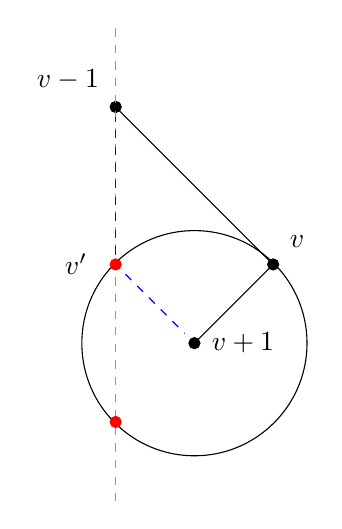
\begin{tikzpicture}
      \node(A) at (0,0) {\pgfuseplotmark{*}};
       \node(NA)[above left = 1pt, outer sep=2pt,fill=white] at (0,0) {$v-1$};
       
       \node(B) at (2,-2) {\pgfuseplotmark{*}};
       \node(NB)[above right = 1pt, outer sep=2pt,fill=white] at (2,-2) {$v$};
       
       \node(C) at (1,-3) {\pgfuseplotmark{*}};
       \node(NC)[right = 1pt, outer sep=2pt,fill=white] at (1,-3) {$v + 1$};
       
       \draw (0,0) -- (2,-2);
       \draw (2,-2) -- (1,-3);
       
       \draw (C) circle [radius=1.43];
       
       \draw[green, dashed] (0,1) -- (0,-5);
       
       \node(P1)[red] at (0, -2) {\pgfuseplotmark{*}};
       \node(VP)[left = 5pt, outer sep=2pt,fill=white] at (0,-2) {$v'$};
       \node[red] at (0, -4) {\pgfuseplotmark{*}};
       
       \draw[blue, dashed] (P1) -- (A);
       \draw[blue, dashed] (P1) -- (C);
     \end{tikzpicture}
     
    \end{enumerate}
     \item Krawędź ma~,,relację'' długości ($L_1$) \\
     Jeśli przesunięcie poprzedniego wierzchołka nie~spowodowało zmiany~długości obecnie przetwarzanej krawędzi,
     to~możemy zakończyć procedurę. W~przeciwnym wypadku, musimy~rozważyć następujące przypadki: 
     \begin{enumerate}
      \item Krawędź $(s+1)-sza$ jest krawędzią bez relacji \\
	Wówczas przesuwamy $v$-ty punkt o~taki sam wektor, o~jaki został przesunięty poprzedni wierzchołek i~kończymy procedurę
      \item Krawędź $(s+1)-sza$ ma relację poziomą \\
       Postępujemy analogicznie do~przypadku \hyperlink{HorLen}{$1c$} z~różnicą, że~środek okręgu będzie w~przesuniętym $(v-1)-szym$ wierzchołku.
      \item Krawędź $(s+1)-sza$ ma relację pionową \\
       Postępujemy analogicznie do~przypadku \hyperlink{VerLen}{$2c$} z~różnicą, że~środek okręgu będzie w~przesuniętym $(v-1)-szym$ wierzchołku.
      \item Krawędź $(s+1)-sza$ ma ustaloną długość ($L_2$) \\
      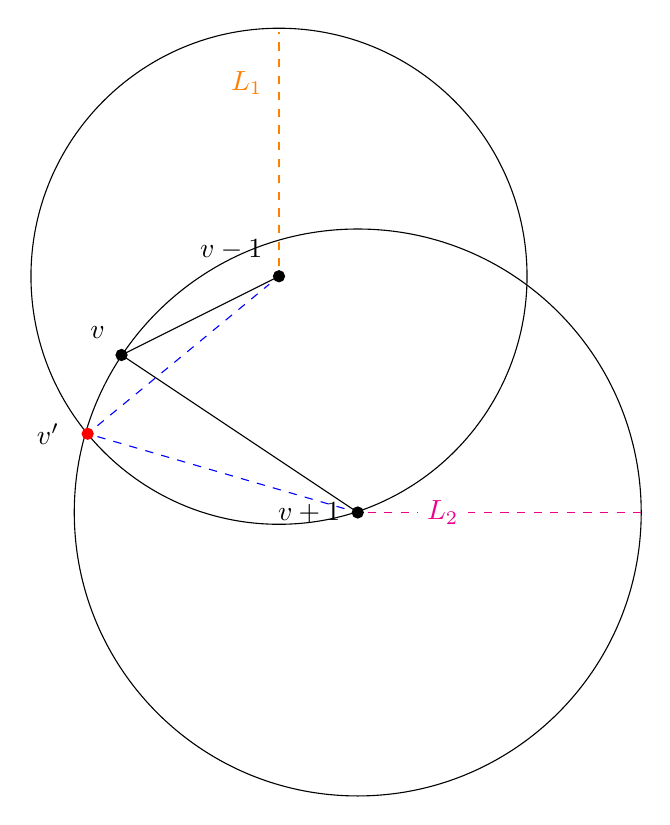
\begin{tikzpicture}
       \node(A) at (0,-1) {\pgfuseplotmark{*}};
       \node(NA)[above left = 1pt, outer sep=2pt,fill=white] at (0,-1) {$v-1$};
       
       \node(B) at (-2,-2) {\pgfuseplotmark{*}};
       \node(NB)[above left = 1pt, outer sep=2pt,fill=white] at (-2,-2) {$v$};
       
       \node(C) at (1,-4) {\pgfuseplotmark{*}};
       \node(NC)[left = 1pt, outer sep=2pt,fill=white] at (1,-4) {$v + 1$};
       
       \draw (0,-1) -- (-2,-2);
       \draw (-2,-2) -- (1,-4);
       
       \draw (A) circle [radius=3.15];
       \draw (C) circle [radius=3.6];
       
       \draw[orange, dashed] (A) --(0, 2.1);
       \node(NN)[orange, above left = 1pt, outer sep=2pt,fill=white] at (0,1.1) {$L_1$};
       
       \draw[magenta, dashed] (C) --(4.6, -4);
       \node(NM)[magenta,  left = 1pt, outer sep=2pt,fill=white] at (2.5,-4) {$L_2$};
       
       \node[red](P1) at (-2.43,-3) {\pgfuseplotmark{*}};
       \node(NP)[left = 5pt, outer sep=2pt,fill=white] at (-2.43,-3) {$v'$};
       
       \draw[blue, dashed] (P1) -- (A);
       \draw[blue, dashed] (P1) -- (C);
       
      \end{tikzpicture} \\
      W~tym przypadku znajdujemy punkty przecięcia dwóch okręgów o~środkach w~$(v-1)$-szym i~$(v+1)$-szym wierzchołku
      i~promieniach równych odpowiednio $L_1$ i~$L_2$. Jeśli~istnieje przynajmniej jeden punkt przecięcia,
      to~znaczy, że~na to miejsce możemy przesunąć wierzchołek $v$-ty i~relacje dla~obydwu krawędzi będą spełnione.
      Wobec~tego, możemy zakończyć procedurę. W~przeciwnym wypadku, jesteśmy zmuszeni przesunąć wierzchołek o~numerze $v$
      o~ten sam wektor, o~który został przesunięty $(v-1)$-szy wierzchołek i~przejść do~przetwarzania kolejnego wierzchołka i~kolejnej
      krawędzi. 	

      
     \end{enumerate}


  \item Puste (krawędź nie ma ustawionej relacji) \\
    To znaczy, że~nie musimy podejmować żadnych kroków i~możemy~zakończyć procedurę ,,naprawczą''.
  
  
 \end{enumerate}
\subsection{Algorytm przesuwania wierzchołka}
Algorytm przesuwania wierzchołka jest bardzo podobny do~algorytmu ustawiania relacji. Różni się tym, że~poprawiamy krawędzie
rozpoczynając od~krawędzi przyległych do~przesuwanego wierzchołka idąc w~obie strony (zgodnie z~ruchem wskazówek zegara,
a~potem przeciwnie do~ruchu wskazówek zegara). Możemy~najpierw obliczyć wektory przesunięcia dla~każdego wierzchołka idąc
zgodnie z~ruchem wskazówek zegara, a~następnie -- idąc przeciwnie. Jeśli istnieje taki wierzchołek (inny od~wierzchołka przesuwanego),
który ma~niezerowy wektor przesunięcia na~obu listach, to~znaczy, że~nie jest możliwe przesunięcie wierzchołka.
 
 

 





\end{document}
